%%%%%%% Studiant Template %%%%%%%
% Template LAB/report ESIEA
%
% Author : Armand ITO

% IN built

%
%%%%%%%%%%%%%%%%%%%%%%%%%%%%%%%%%

% Kind of base document and option
\documentclass[answers,a4paper,twoside]{School-Work-Template}



\Title{Type de documents}{\textit{version : 1.0}}


\author{
	\begin{tabular}[t]{p{0.4\textwidth}@{\extracolsep{2em}}p{0.4\textwidth}}
		\rule{0.8\textwidth}{0.4pt}\vspace{1cm}\\
		\centering Lorem Ipsum 2 $^1$  & \centering  Lorem Ipsum 2 $^2$ \tabularnewline
		\centering  \includegraphics[width=0.4\textwidth]{example-image-a} & \centering  \includegraphics[width=0.4\textwidth]{example-image-b} \tabularnewline
		Quisque dolor mi, pulvinar venenatis placerat sed, semper posuere nibh. Nam dapibus lacus eget nulla auctor in velit. & Quisque dolor mi, pulvinar venenatis placerat sed, semper posuere nibh. Nam dapibus lacus eget nulla auctor in velit.
	\end{tabular}\vspace{1.5cm}\\
	\begin{tabular}[t]{p{0.3\textwidth}@{\extracolsep{2em}}p{0.3\textwidth}@{\extracolsep{2em}}p{0.3\textwidth}}
		\textbf{Maître de stage} :&\textbf{Tuteur pédagogique} : & \textbf{Stagiaire} :\vspace{0.3cm}\\
		Monsieur & Monsieur & Monsieur\\
		\hspace{0.2cm}X Y, &\hspace{0.2cm}X Y, &\hspace{0.2cm}X Y,\\
		\hspace{0.2cm}\small X Y & \hspace{0.2cm}\small X Y & \hspace{0.2cm}\small X Y\vspace{1cm}\\
		Lu et approuvé :& Lu et approuvé : & Lu et approuvé :
	\end{tabular}
	\thispagestyle{empty}           		
}

% Abstract Contant
\abs{...}

\begin{document}
\oddsidemargin=1.15cm

\backgroundsetup{contents={},scale=1,placement=top,opacity=1,position={6cm,2.2cm}}
\thispagestyle{empty}
\AddToShipoutPicture*{\AtPageLowerLeft{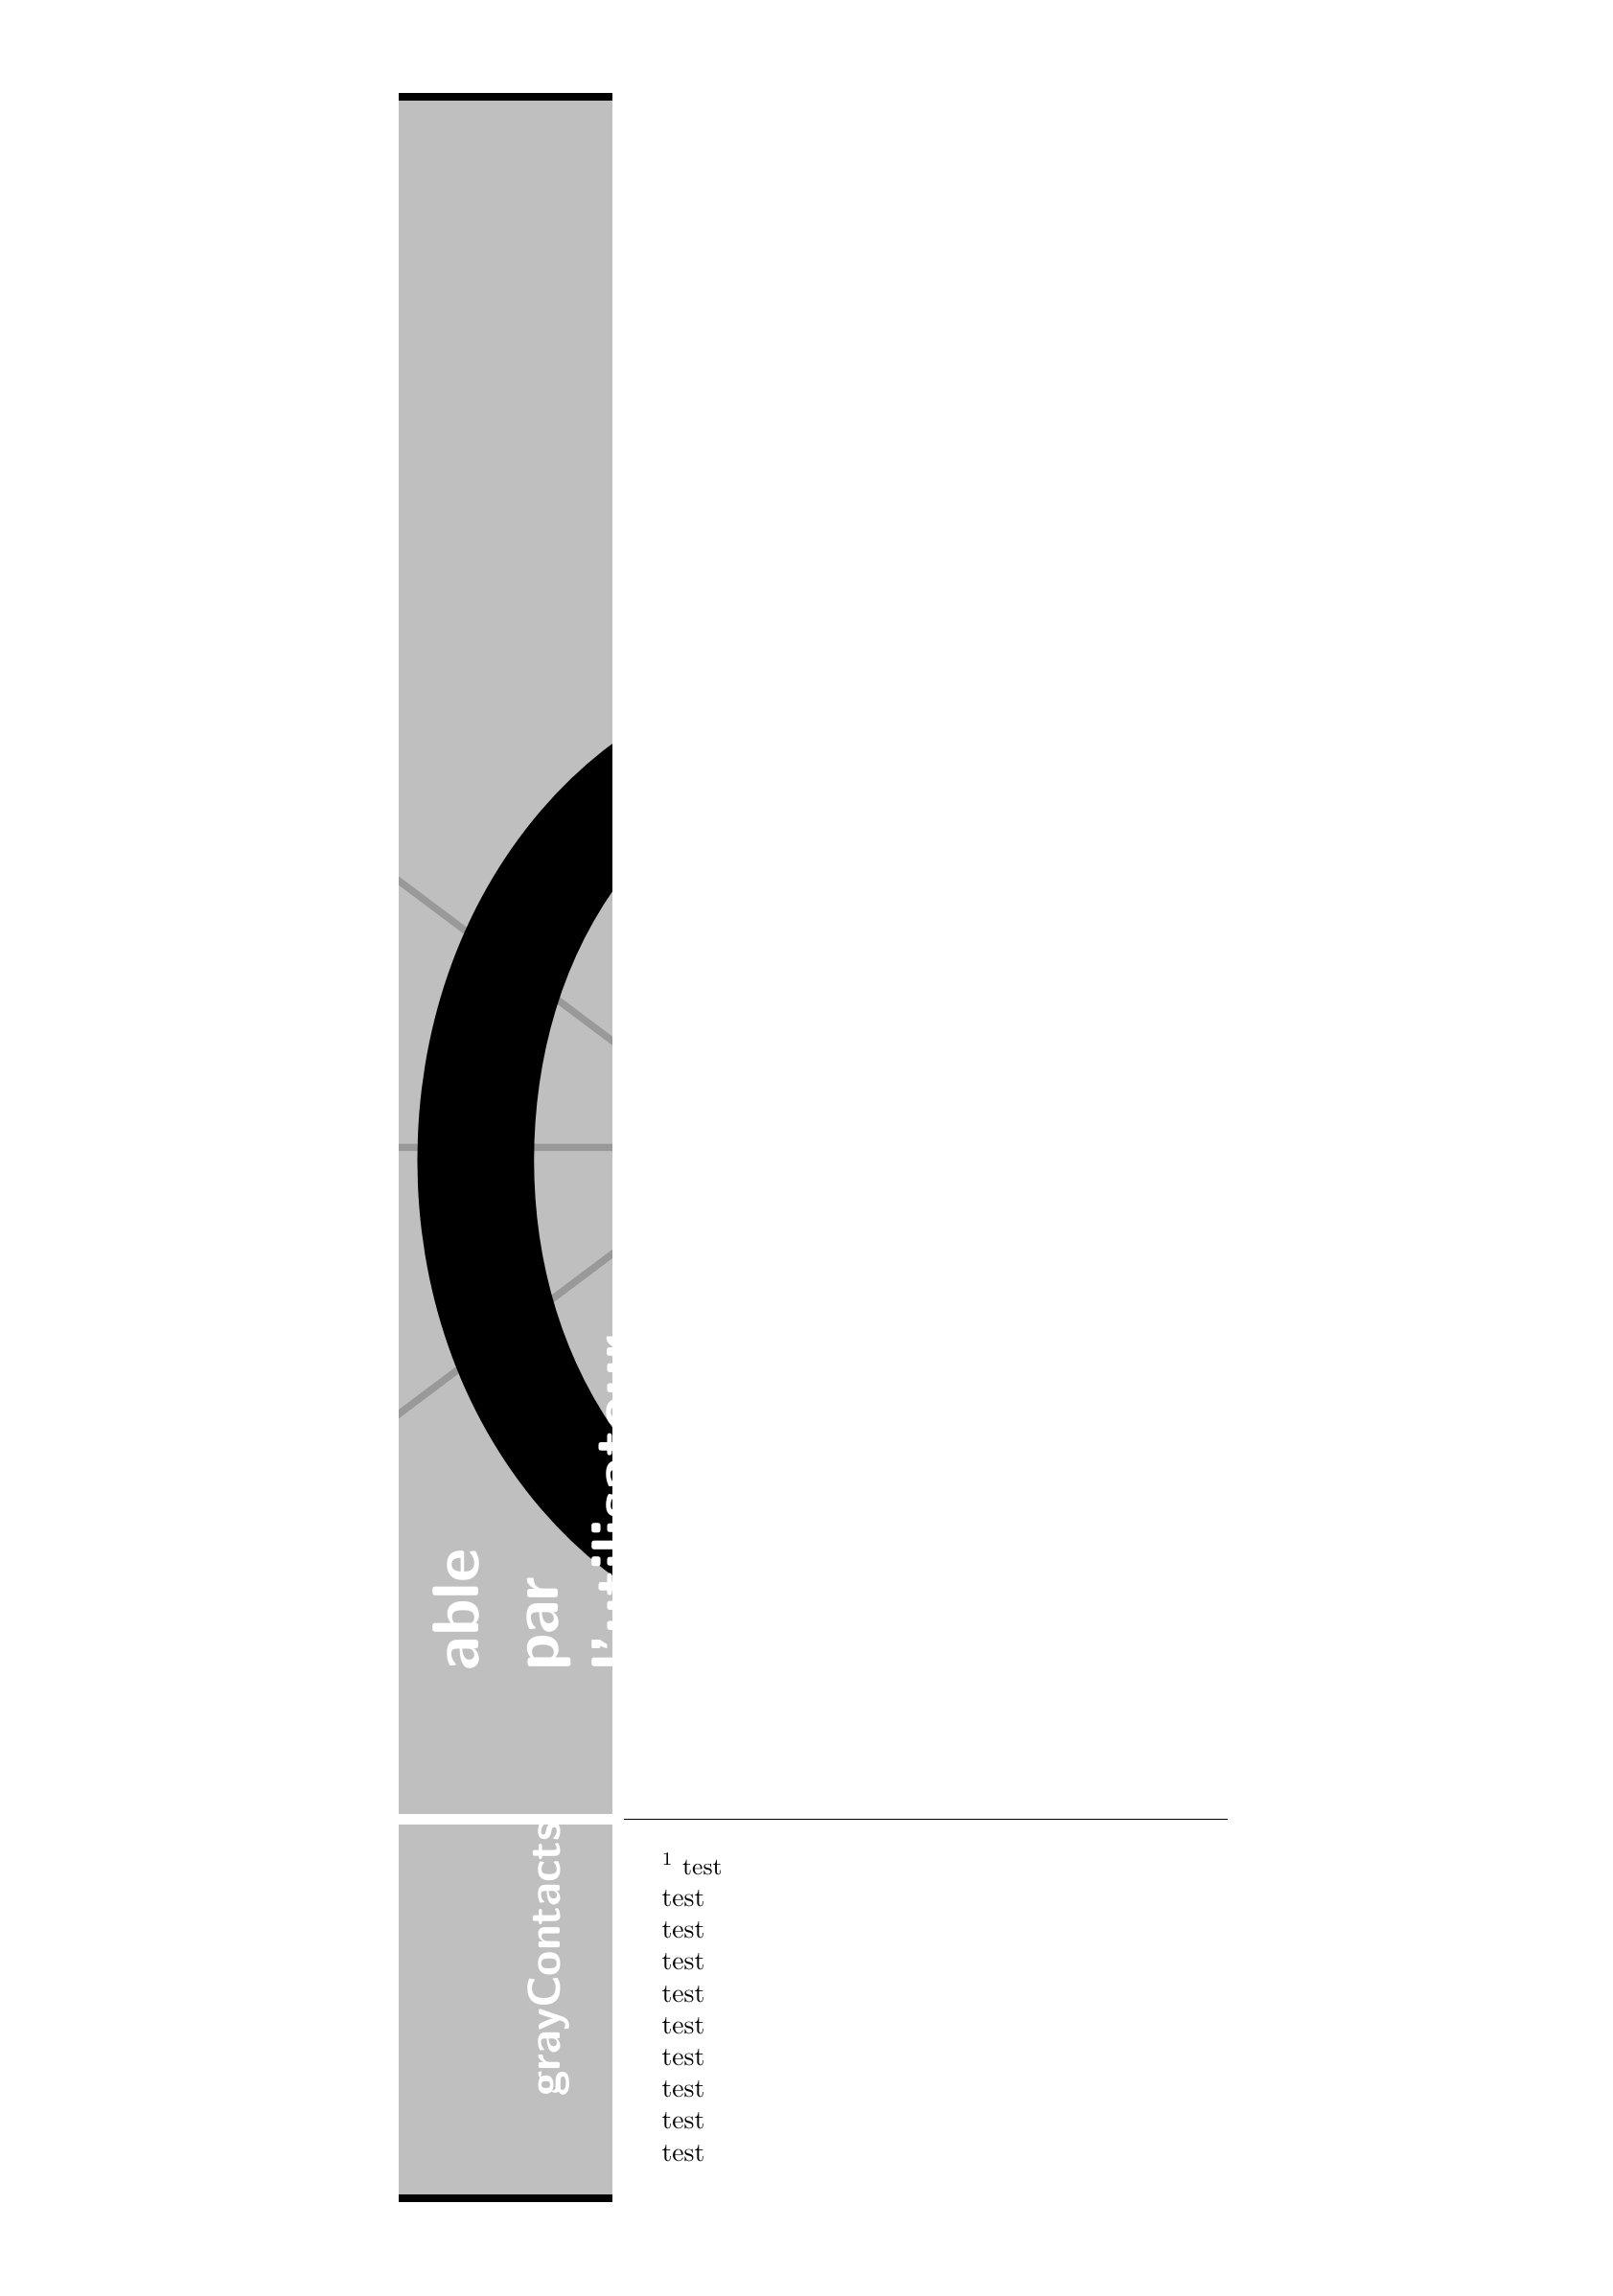
\begin{tikzpicture}
	\draw[ white, path picture = {\node [] at (path picture bounding box.center) {\includegraphics[height=\paperheight,trim=-2cm 0 0 0]{example-image-c}}; } ] (-.5,0)rectangle(2.35,29.70);
	\draw[ white, very thick,fill](-.5,6)rectangle (2.35,5.9);
	%\node[rotate=90,color=white,text width=5,align=left] at (1,8) {\Huge{\sffamily\textbf{\contour{gray}{\color{white}Sélection d'une plateforme de virtualisation}}}\\ \Huge{\sffamily\textbf{\contour{gray}{\color{white}en systèmes embarqués }}} \\ \Huge{\sffamily\textbf{\contour{gray}{\color{white}en systèmes embarqués }}} };
	\node[rotate=90,color=white,text width=5,align=left] at (1,8) {\Huge{\sffamily\textbf{\contour{gray}{\color{white}Long titre modifiable par l'utilisateur}}}\\ \Huge{\sffamily\textbf{\contour{gray}{\color{white}seconde lignes modifiable }}}};
	\node[rotate=90,color=white] at (1.5, 4) {\LARGE{ \sffamily\textbf{\contour{gray}{\color{white}Contacts}}}};
	\node at (6.5,5.95){\rule{8cm}{0.4pt}};
	\node[] (contact) at (3,5.5) {} ;
	\node[below right, text width=\textwidth] at (contact.north west) {$^1$ {\small test} \\ test \\ test \\ test \\ test \\ test \\ test \\ test \\ test \\ test };;
	\end{tikzpicture}}}
\maketitle

\newpage
\thispagestyle{empty}

% blank page
\newpage
\backgroundsetup{contents={},scale=1,placement=top,opacity=1,position={6cm,2.2cm}}
\null
\thispagestyle{empty}%
%\addtocounter{page}{-2}%

%%%%%%%%%%% DOCUMENT MAIN CONTENT

%% write your document here %%
%% ↓ example %%

% Aesthetic spacing redefines that look nicer to me than the defaults.
\newpage
\thispagestyle{empty}
\begin{center}
	\textbf{{\Large Remerciement}}
\end{center}
...
\newpage
\thispagestyle{empty}
\section*{Abstract}%
...
\newpage
\thispagestyle{empty}
\section*{Résumé}%
...
\newpage
\tableofcontents


\newpage
\chapter{Partie Une}
\section{Démarche}
Cette  réalisation s'effectuera en plusieurs étapes:
\begin{itemize}
	\item Étude théorique
	\begin{itemize}
		\item[$\circ$] Modélisation du système et identification.
		\item[$\circ$] Réponse statique et dynamique du système.
		\item[$\circ$] Calcul d'un correcteur  P.I.D en vue d'obtenir le meilleur compromis stabilité/temps de réponse.
		\item[$\circ$] Réponse statique et dynamique du système corrigé.
	\end{itemize}
	\item Étude expérimentale reprenant les points de l'étude théorique.
	\item Comparaison des résultats. 
\end{itemize}
\newpage
\section{Système}
\subsection{Matérielle mise à disposition}

%\begin{figure}[h!]
%	\centering
%	\begin{tikzpicture}
%	\node[anchor=south west,inner sep=0] (image) at (0,0) {\includegraphics[scale=0.25,bb=0 0 30 30]{img/P1.jpg}
%	\includegraphics[scale=0.25,bb=0 0 30 30]{img/P2.jpg}};
%	\begin{scope}[x={(image.south east)},y={(image.north west)}]
	
%	\node[draw,rectangle,dashed,red,ultra thick,rounded corners,minimum width=5mm,minimum height=8mm] (Jumper) at (0.315,0.42){ };
%	\coordinate (Moter) at (0.215,0.6);
%	\coordinate (Reduct) at (0.2,0.68);
%	\coordinate (Ampli-GND) at (0.22,0.1);
%	\coordinate (Ampli-minus) at (0.29,0.1);
%	\coordinate (Ampli-plus) at (0.14,0.1);
%	\coordinate (Input) at (0.22,0.05);
%	\coordinate (Pot) at (0.91,0.4);
%	\coordinate (AlimPot-plus) at (0.85,0.4);
%	\coordinate (Output) at (0.85,0.35);
%	\coordinate (AlimPot-minus) at (0.85,0.3);
%	\coordinate (Disque1) at (0.8,0.55);
%	\coordinate (Disque2) at (0.35,0.93);
	
%	\node (N-Jumper) at (-0.25,0.42) {\sffamily Jumper};
%	\draw[->,line width=0.25mm,red]  (N-Jumper) -- (Jumper.west);
	
%	\node (N-Moter) at (-0.25,0.6) {\sffamily Moteur};
%	\draw[->,line width=0.25mm,red]  (N-Moter) -- (Moter.west);
	
	
%	\node (N-Reduct) at (-0.25,0.7) {\sffamily Réducteur};
%	\draw[->,line width=0.25mm,red]  (N-Reduct) -- (Reduct.west);
	
%	\node[text width=2.7cm] (N-Ampli) at (-0.25,0.2) {\sffamily Alimentation de l'Amplificateur};
%	\draw[->,line width=0.25mm,red]  (N-Ampli.east) -- (Ampli-GND.west);
%	\draw[->,line width=0.25mm,red]  (N-Ampli.east) -- (Ampli-plus.west);
%	\draw[->,line width=0.25mm,red]  (N-Ampli.east) -- (Ampli-minus.west);
	
%	\node (N-Input) at (-0.25,0.06) {\sffamily Entrée};
%	\draw[->,line width=0.25mm,red]  (N-Input.east) -- (Input.west);
	
%	\node (N-Disque) at (1.2,0.8) {\sffamily Disque};
%	\draw[->,line width=0.25mm,red]  (N-Disque.west) -- (Disque1.west);
%	\draw[->,line width=0.25mm,red]  (N-Disque.west) -- (Disque2.west);
	
%	\node (N-Pot) at (1.2,0.4) {\sffamily Potentiomètre};
%	\draw[->,line width=0.25mm,red]  (N-Pot.west) -- (Pot.west);
	
%	\node (N-Output) at (1.2,0.3) {\sffamily Sortie};
%	\draw[->,line width=0.25mm,red]  (N-Output.west) -- (Output.west);
	
%	\node[text width=2.7cm]  (N-Alim) at (1.2,0.15) {\sffamily Alimentation du Potentiomètre};
%	\draw[->,line width=0.25mm,red]  (N-Alim.west) -- (AlimPot-plus.west);
%	\draw[->,line width=0.25mm,red]  (N-Alim.west) -- (AlimPot-minus.west);
	
%	\end{scope}
%	\end{tikzpicture}
%	\caption{Photo du système étudier}
%\end{figure}
%\noindent
Comme on peut le voir sur la Figure 2 le dispositif est composé :

\begin{itemize}
	\item D'un amplificateur de courant ;
	\item D'un moteur lié mécaniquement à un réducteur de rapport 15 lui même lié à une charge connecté au disque sur un même axe;
	\item D'un disque avec marque jaune (adhésif);
	\item D'un potentiomètre permettant de mesurer la position angulaire.
\end{itemize}

\newpage
\subsection{Description du système}

\noindent
Modélisé en un système automatique l'on peut résumer ce dispositif par un système à boucle (voir Figure 3 ).

\begin{figure}[h!]
	\centering
	\begin{tikzpicture}
	\sbEntree{ve}
	\sbComp{a}{ve}
	\sbBloc{b}{Ad}{a}
	\sbRelier[$V_e$]{ve}{a}
	\sbBlocL{c}{Moteur}{b}
	\sbRelier[$\varepsilon$]{a}{b}
	\sbRelier[$U$]{b}{c}
	%\sbComph{e}{c}
	%\sbRelier[u]{c}{d}
	\sbBlocL{d}{Réducteur}{c}
	\sbRelier[$\theta_e$]{c}{d}
	\sbBlocL{e}{Charge}{d}
	\sbRelier[$\theta_s$]{d}{e}
	\sbSortie[3]{S1}{e}
	\sbRelier{e}{S1}
	\sbNomLien[0.8]{S1}{$\theta_s$}
	%\sbDecaleNoeudy[-4]{e}{u}
	\sbDecaleNoeudy{d-e}{v}
	%\sbBlocr{r1}{$R_1$}{u}
	\sbBlocr{r2}{Potentiomètre}{v}
	\sbBlocrL{r3}{Ab}{r2}
	%\sbRelieryx{e-S1}{r1}
	%\sbRelierxy[n1]{r1}{d}
	\sbRelieryx{e-S1}{r2}
	\sbRelierxy{r3}{a}
	\end{tikzpicture}
	\caption{Schéma bloc de l'asservissement d'un disque}
\end{figure}
\noindent
Ad et Ab sont des amplificateurs de tension de gain indépendant de la fréquence.
\vspace{0.5cm}\\
\noindent
La sortie de ce réducteur  est couplée  à un disque faisant office de charge et à un potentiomètre qui fournit une tension proportionnelle à la position du disque. 

\subsection{Fonctionnement du potentiomètre}

\begin{figure}[h!]
	\centering
	\begin{tikzpicture}[scale=2.5]
	
	% center c2
	\coordinate (c) at (0,0);
	
	\draw [blue!50,fill] (c) circle [radius=0.5mm];
	
	\draw [dashed] (c) circle [radius=7mm];
	
	\draw[fill=gray!50]
	% radius=5mm, initial=45, final=270
	($(c) + (-80:5mm)$) arc (-80:260:5mm)
	--
	% radius=6mm, reversed
	($(c) + (260:6mm)$) arc (260:-80:6mm)
	-- cycle;
	
	\draw [blue!50,fill] (45:5.5mm) circle [radius=0.35mm] ;
	
	\draw[blue!50, line width=0.5mm] (45:5.5mm) coordinate (mary) -- (c) ;
	
	\draw [red,fill] (260:5.5mm) circle [radius=0.25mm];
	
	\draw [green,fill] (-80:5.5mm) circle [radius=0.25mm];
	
	\coordinate (p15) at (260:5.5mm);\vspace{-3cm}
	\coordinate (m15) at (-80:5.5mm);
	
	\coordinate[below of= p15] (a);
	\coordinate[below of= m15] (b);
	
	\draw[red] (p15) -- (a);
	\draw[green] (m15) -- (b);
	
	\node[left of=a] (m) {+15V};
	\draw[red] (a) -- (m);
	
	\node[right of=b] (g) {-15V};
	\draw[green] (g) -- (b);
	
	\node[below of=c,node distance=3cm] (Vs) {$V_{output}$};
	\draw[blue!50, line width=0.5mm] (Vs) coordinate (bob) -- (c) ;
	
	\pic [draw, ->, "$\theta_s$", angle eccentricity=1.5] {angle = bob--c--mary};
	
	\end{tikzpicture}
	\caption{ Illustration d'un potentiomètre}
\end{figure}

\noindent
Le potentiomètre dispose d'une piste de $10$K$\Omega$.\\
\noindent
La résistance de sortie varie entre $0$ et $2.5$ K$\Omega$, avec $0$K$\Omega$ lorsque $
\theta_s\simeq\dfrac{3\pi}{2}+2K\pi$ et $2.5$K$\Omega$ quant $
\theta_s\simeq\dfrac{\pi}{2}+2K\pi$.

\newpage
\subsection{Fonctionnement du réducteur}



\begin{figure}[h!]
	\centering
	\begin{tikzpicture}[scale=1.5]
	\coordinate (c) at (0,0);
	\draw[dashed] (-2.5,0)--(c)--(3.5,0);
	
	\coordinate (c1) at (1.5,0);
	\coordinate (c2) at (-1,0);
	
	\draw (c1) circle [radius=1.5cm];
	\draw[line width=0.5mm] (1.5,0.15)--(1.5,-0.15);
	\draw[line width=0.5mm] (1.35,0)--(1.65,-0);
	\node[below of=c1,node distance=0.5cm]{($R_s$,$Z_s$)};
	\draw[->,>=stealth',semithick,pin=22] ($(c1) + (70:1.7cm)$) arc (70:30:1.7cm) node[above=0.25cm] {$\omega_s$} ;
	
	\node[below right of=c1,node distance=4cm,text width=3.8cm] {\textbf{Sortie} (récepteur): roue \textbf{menée}};
	
	\draw (c2) circle [radius=1cm];
	\draw[line width=0.5mm] (-1,0.15)--(-1,-0.15);
	\draw[line width=0.5mm] (-1.15,0)--(-0.85,-0);
	\node[below of=c2,node distance=0.5cm]{($R_e$,$Z_e$)};
	
	\draw[->,>=stealth',semithick,pin=22] ($(c2) + (95:1.2cm)$) arc (95:140:1.2cm) node[above=0.25cm] {$\omega_e$} ;
	
	
	\node[below of=c2,node distance=2.8cm,text width=3.8cm] {\textbf{Entrée} (moteur): pignon \textbf{menant}};
	
	\end{tikzpicture}
	\caption{Illustration de Pignon droit}
\end{figure}

\underline{\textcolor{red}{Définition :}}

\noindent
Un réducteur est un système d'engrenages dont le rapport de transmission est inférieur à 1, pour augmenter le couple moteur d'une rotation ou pour réduire la vitesse.
\vspace{0.25cm}\\
\noindent 
Il existe aussi des réducteurs en L pour modifier l'angle de sortie. 
\vspace{0.25cm}\\
\noindent
En soit un réducteur mécanique a pour but de modifier le rapport de vitesse ou/et le couple entre l'axe d'entrée et l'axe de sortie d'un mécanisme (exemple voir Figure 5).
\newpage
\subsection{Fonctionnement de l'amplificateur de puissance}

\noindent
Dans un amplificateur de puissance les transistors T1 et T2 sont placés en sortie de l'AOP pour amplifier le courant délivré à la charge.

% TODO : réécrir avec ses propre mots
\begin{figure}[h!]
	\centering
	\tikz \node [scale=0.75, inner sep=0] {
		\shorthandoff{:!}
		\begin{circuitikz}
			
			\draw (2,1) node[op amp] (opamp1) {} 
			(0.8,0) node [cground] {}  |- (opamp1.+)
			(opamp1.out) to[short] (4,1);
			\draw[gray]	(opamp1.-) -| +(0,5) to[generic,l=$R2$] +(4,5) -|  (7,1);
			
			\draw (-1,1.5)node[left,xshift=-0.25cm]{$V_e$} to[short,o-] (-0.75,1.5) to[generic,l=$R1$] (opamp1.-); 
			
			\draw (10,6)node[right,xshift=0.25cm]{$+15$} to[short,o-] (4,6) to[generic,l=$R3$]  (4,3.5) to[Do,l=$D1$] (4,2) to [short] (4,1);
			
			\draw (10,-4)node[right,xshift=0.25cm]{$-15$} to[short,o-] (4,-4) to[generic,l=$R4$]  (4,-1.5) (4,0)to[Do,l=$D4$] (4,-1.5) 
			(4,0) to [short] (4,1);
			
			\draw (6,3.75) node[npn](T1){$T1$} 
			(6,6) to[short] (T1.C) 
			(4,3.75) to[short] (T1.B) 
			(T1.E)  to[generic,l=$R5$] (6,1)
			;
			
			\draw (6,-1.75) node[pnp](T2){$T2$}
			(6,-4) to[short] (T2.C) 
			(4,-1.75) to[short] (T2.B)
			(T2.E) to[generic,l=$R6$] (6,1);
			
			\draw (6,1) to[short,-o] (9,1)  node[right,xshift=0.25cm]{$V_s$}
			(8,1) to[generic,l=$\ charge$] (8,-1)  node [cground] {} ;
			
			\draw (8,-4) to[ecapacitor] (8,-6)node [cground] {}
			(9,-4) to[C] (9,-6)node [cground] {};
			
			\draw (8,6) to[ecapacitor] (8,4)node [cground] {}
			(9,6) to[C] (9,4)node [cground] {};
			
		\end{circuitikz}
	};
	\caption{Montage avec polarisation de l'étage de sortie}
\end{figure}

\noindent
L'AOP amplifie en tension avec le gain -R2/R1. L'amplificateur de courant de sortie est constitué par les éléments R3, D1, D2, R4, T1, R5, R6 et T2. Le courant délivré en sortie de l'AOP est amplifié par les transistors T1 et T2. L'alternance positive est délivrée par le transistor T1 tandis que l'alternance négative l'est par T2.
\vspace{0.25cm}

\noindent
Le rôle de R3, D1, D2 et R4 est de polariser les transistors. Le courant continu de sortie de repos (en l'absence de tension de sortie) est ajusté par les tensions aux bornes des diodes D1 et D2.  Quand les résistances R4 et R5 sont réduites, la tension aux bornes de D1 et D2 augmente et il en est de même pour le courant de repos dans R5 et R6.
\vspace{0.25cm}


\noindent
R5 et R6 jouent un rôle de stabilisation thermique. En effet, quand la tension Vbe aux bornes des transistors T1 et T2 varie suite à une variation de la température (la puissance délivrée par T1 et T2 peut ne pas être négligeable et il y a échauffement des transistors), le courant de repos dans les transistors augmente et il en est de même pour les tensions aux bornes de R5 et R6. Comme la tension aux bornes de D1 et D2 varie peu, les tensions Vbe vont être réduite.
\vspace{0.25cm}


\noindent
La contre réaction de l'AOP est faite après les deux transistors pour avoir une tension avec peu de distorsion en sortie.
\vspace{0.25cm}


\noindent
Ne pas oublier de découpler les alimentations +15 V et - 15 V par deux capacités chimiques et plastiques en parallèle comme indiqué sur la figure 6. Attention au sens des capacités chimiques.

\newpage
\subsection{Spécificité technique}
% TODO : compléter la liste ci-dessous

\begin{itemize}
	\item Jumper : Le système dispose d'un Jumper permettant au étudiant de coupé l'injection de courant vers le disque en cas de problème ;
	\item Disque : 
	\item Réducteur :
	\item Moteur :
	\item Potentiomètre :
	\item Amplificateur :
\end{itemize}

\newpage
\section{Théorique}
\subsection{Méthode par calcul théorique en utilisant le PFD}
\subsubsection{Relation relatives au moteur}
\subsubsection{Équations relatives au réducteur (supposé sans pertes)}

\subsection{diagramme PERT}

\begin{figure}[h!]
	\centering
	
	\tikzset{nodePERT/.style={draw,circle, append after command={
				[shorten >=\pgflinewidth, shorten <=\pgflinewidth,]
				([yshift=0.2mm]\tikzlastnode.base) edge  ([yshift=0.4mm]\tikzlastnode.south)
				([xshift=-0.4mm]\tikzlastnode.east) edge  ([xshift=0.4mm]\tikzlastnode.west)
			}
		}
	}
	\tikzset{line/.style={very thick,->,>=stealth'}}
	\tikzset{radius/.style={very thick,-,>=stealth'}}
	
	\tikzset{figtive/.style={->,>=stealth',thick,dashed}}
	\tikzset{cp/.style={double,double equal sign distance,-implies}}
	
	
	\begin{tikzpicture}[thick,scale=1.15, every node/.style={transform shape}]
	%node 0
	\node (nodePERT-aa)[nodePERT, fill=white, scale=4] {};
	\node[above=-0.65cm] at (nodePERT-aa.north) {0};
	\node[below left] at (nodePERT-aa) {0};
	\node[below right] at (nodePERT-aa) {0};
	
	%node 1
	\node (nodePERT-bb)[nodePERT,right of=nodePERT-aa,above=3cm ,node distance=4cm, scale=4] {};
	\node[above=-0.65cm] at (nodePERT-bb.north) {1};
	\node[below left] at (nodePERT-bb) {6};
	\node[below right] at (nodePERT-bb) {9};
	
	%node 2
	\node (nodePERT-cc)[nodePERT,right of=nodePERT-aa,above=1cm ,node distance=3cm, fill=white, scale=4] {};
	\node[above=-0.65cm] at (nodePERT-cc.north) {2};
	\node[below left] at (nodePERT-cc) {9};
	\node[below right] at (nodePERT-cc) {12};
	
	%node 3
	\node (nodePERT-dd)[nodePERT,right of=nodePERT-aa,below=1cm ,node distance=3cm, fill=white, scale=4] {};
	\node[above=-0.65cm] at (nodePERT-dd.north) {3};
	\node[below left] at (nodePERT-dd) {4};
	\node[below right] at (nodePERT-dd) {12};
	
	%node 4
	\node (nodePERT-ee)[nodePERT,right of=nodePERT-aa,below=3cm ,node distance=4cm, fill=white, scale=4] {};
	\node[above=-0.65cm] at (nodePERT-ee.north) {4};
	\node[below left] at (nodePERT-ee) {7};
	\node[below right] at (nodePERT-ee) {7};
	
	%node 5
	\node (nodePERT-ff)[nodePERT,right of=nodePERT-aa ,node distance=6.5cm, fill=white, scale=4] {};
	\node[above=-0.65cm] at (nodePERT-ff.north) {5};
	\node[below left] at (nodePERT-ff) {12};
	\node[below right] at (nodePERT-ff) {12};
	
	%node 6
	\node (nodePERT-gg)[nodePERT,right of=nodePERT-aa,above=3cm ,node distance=9cm, fill=white, scale=4] {};
	\node[above=-0.65cm] at (nodePERT-gg.north) {6};
	\node[below left] at (nodePERT-gg) {17};
	\node[below right] at (nodePERT-gg) {18};
	
	%node 7
	\node (nodePERT-hh)[nodePERT,right of=nodePERT-aa,below=3cm ,node distance=9cm, fill=white, scale=4] {};
	\node[above=-0.65cm] at (nodePERT-hh.north) {7};
	\node[below left] at (nodePERT-hh) {16};
	\node[below right] at (nodePERT-hh) {16};
	
	%node 8
	\node (nodePERT-ii)[nodePERT,right of=nodePERT-aa ,node distance=12cm, fill=white, scale=4] {};
	\node[above=-0.65cm] at (nodePERT-ii.north) {8};
	\node[below left] at (nodePERT-ii) {21};
	\node[below right] at (nodePERT-ii) {21};
	
	% coodonate 1
	\coordinate [right of=nodePERT-aa,above=3.7cm ,node distance=1.5cm] (coordonate1);
	
	% coodonate 2
	\coordinate [right of=nodePERT-aa,above=1.7cm ,node distance=1.25cm] (coordonate2);
	
	% coodonate 3
	\coordinate [right of=nodePERT-aa,below=1.7cm ,node distance=1.25cm] (coordonate3);
	
	% coodonate 4
	\coordinate [right of=nodePERT-aa,below=3.7cm ,node distance=1.5cm] (coordonate4);
	
	% A' task
	\draw[line] (nodePERT-aa) -- (coordonate1) -- node [above] {$A'$} node [below] {6} (nodePERT-bb);
	
	% B task
	\draw[line] (nodePERT-aa) -- (coordonate2) --  node [above] {$B$} node [below] {9} (nodePERT-cc);
	
	% C task
	\draw[line] (nodePERT-aa) --  node [above] {$C$} node [below] {11} (nodePERT-ff);
	
	% D task
	\draw[line] (nodePERT-aa) -- (coordonate3) -- node [above] {$D$} node [below] {4} (nodePERT-dd);
	
	% E' task
	\draw[cp] (nodePERT-aa) -- (coordonate4) -- node [above] {$E'$} node [below] {7} (nodePERT-ee);
	
	
	% A'' task
	\draw[line] (nodePERT-bb) --  node [above] {$A''$} node [below] {4} (nodePERT-gg);
	
	% E'' task
	\draw[line] (nodePERT-ee) --  node [above] {$E''$} node [below] {7} (nodePERT-hh);
	
	
	% figtive1 task
	\draw[figtive] (nodePERT-cc) --  node [below] {$\varnothing$}  (nodePERT-ff);
	
	% figtive2 task
	\draw[figtive] (nodePERT-dd) --  node [above] {$\varnothing$} (nodePERT-ff);
	
	
	
	% F task
	\draw[line] (nodePERT-bb) --  node [above right] {$F$} node [below left] {3} (nodePERT-ff);
	
	% G task
	\draw[cp] (nodePERT-ee) --  node [above left] {$G$} node [below right] {5} (nodePERT-ff);
	
	
	% J task
	\draw[line] (nodePERT-ff) --  node [above] {$J$} node [below] {6} (nodePERT-ii);
	
	% H task
	\draw[line] (nodePERT-ff) --  node [above left] {$H$} node [below right] {5} (nodePERT-gg);
	
	% K task
	\draw[cp] (nodePERT-ff) --  node [above right] {$K$} node [below left] {4} (nodePERT-hh);
	
	% I task
	\draw[line] (nodePERT-gg) --  node [above right] {$I$} node [below left] {3} (nodePERT-ii);
	
	% L task
	\draw[cp] (nodePERT-hh) --  node [above left] {$L$} node [below right] {5} (nodePERT-ii);
	
	\end{tikzpicture}
	\caption{Diagramme PERT du projet EADS}
\end{figure}

\newpage
\subsection{TP d'automatique}

\begin{figure}[h!]
	\centering
	\begin{tikzpicture}
	
	\pgfmathdeclarefunction{p}{1}{%
		\pgfmathparse{(and(#1>-0.2, #1<10))}%
	}
	
	\begin{axis}[title={\sffamily Réponse indicielle d'un système du second ordre $0 < \zeta < 1$},  
	height=0.3\textheight,
	width=0.85\textwidth,
	xlabel={$t$},
	ylabel={$y_1(t)$},
	xtick={0, 0.5, ..., 3},
	ytick={0, 0.2, ..., 1.2},
	xmin=0, xmax=3,
	ymin=0, ymax=1.2,
	domain=0:3,
	grid=major, % Display a grid
	grid style={dotted,gray!50}, % set the style
	legend style={draw=none,at={(0.75,0.25)},anchor=north},
	legend cell align=left
	]
	
	\addplot[dashed]{1};
	
	\addlegendentry{Asymptote}
	
	
	\addplot[color=red,smooth,
	thick,
	mark=none,
	samples=500,domain=0:2*pi]{
		%(1-(e^(-0.5*5*x)/sqrt(1-(0.5)^2) * (\sin(sqrt(1-(0.5)^2)*5*x)*0.5+\cos(sqrt(1-(0.5)^2)*5*x)*sqrt(1-(0.5)^2)) ) 
		(1-(e^(-0.5*5*x)/sqrt(1-(0.5)^2) *(sin(sqrt(1-(0.5)^2)*5*deg(x))*0.5+cos(sqrt(1-(0.5)^2)*5*deg(x))*sqrt(1-(0.5)^2))
	};
	\addlegendentry{Réponse indicielle $y_1(t)$}
	
	\draw [densely dashed] ({rel axis cs:0,0} -| {axis cs:1.45,0})  -- ({rel axis cs:0,0.81} -| {axis cs:1.45,0})  ;	
	\draw [densely dashed] ({rel axis cs:0,0} -| {axis cs:0.72,0}) -- ({rel axis cs:0,0.97} -| {axis cs:0.72,0})  ;	
	
	\end{axis}
	
	\node[] at (2.879, 0) (a) {$\bullet$};
	\node[below left=0cm and -0.60cm of a]{$t_m$};
	
	\node[] at (5.779, 0) (b) {$\bullet$};
	\node[above left=0cm and 0cm of b]{$t_a$};
	\end{tikzpicture}
	\caption{\sffamily Réponse indicielle d'un système du second ordre $0 < \zeta < 1$}
\end{figure}
\newpage
\chapter{Partie test}
\section{test}
...
\chapter{Partie test}
\section{test}
...
\chapter{Partie test}
\section{test}
...
\chapter{Partie test}
\section{test}
...
\chapter{Partie test}
\section{test}
...
\chapter{Partie test}
\section{test}
...
\chapter{Partie test}
\section{test}
...
\chapter{Partie test}
\section{test}
...
\section{test}
...
\section{test}
...
\section{test}
...
\section{test}
...
\section{test}
...
\section{test}
...
\section{test}
...
\section{test}
...
\section{test}
...
\section{test}
...
\section{test}
...
\section{test}
...
\section{test}
...
\section{test}
...
\section{test}
...
\section{test}
...
\section{test}
...
\section{test}
...
\section{test}
...
\section{test}
...
\section{test}
...

\end{document}
